%%%%%%%%%%%%%%%%%%%%%%%%%%%%%%%%%%%%%%%%%%%%%%%%%%%%%%%%%%%%%%%%%%%%%%
%% all the formatting stuff and packages

\documentclass[11pt]{article}

\parindent0em
\parskip.5em

\usepackage{xstring}

\usepackage{amsthm}
\usepackage[utf8]{inputenc}
\usepackage[ttscale=.85]{libertine}
\usepackage{libertinust1math}
% \usepackage[libertine,cmintegrals,cmbraces,vvarbb]{newtxmath}
\usepackage[T1]{fontenc}
\usepackage{microtype}
\usepackage{amsmath}
\usepackage{amssymb}
\usepackage{xspace}
\usepackage{ngerman}
\usepackage{graphicx}
\usepackage{lastpage}
\usepackage{ifthen}
\usepackage{fp}
\usepackage{hyperref}
\usepackage{icomma}
\usepackage{paralist}
\usepackage[ngerman,onelanguage,noend]{algorithm2e}
\DontPrintSemicolon

\makeatletter
\DeclareRobustCommand{\bfseries}{%
   \not@math@alphabet\bfseries\mathbf
   \fontseries\bfdefault\selectfont
   \boldmath
}
\makeatother

\usepackage[headsep=1cm]{geometry}

\usepackage{fancyhdr}

\fancypagestyle{plain}{%
  \renewcommand{\headrulewidth}{0pt}%
  \fancyhf{}
  \rhead{
\includegraphics[width = 2.4cm]{fig/hpi_logo.pdf}}
  \lhead{\textbf{\sffamily Parametrisierte Algorithmen} \\
    \textbf{\sffamily Wintersemester 2017/2018} \\
    \sffamily Thomas Bläsius}
  \cfoot{\thepage}
  \rfoot{\ifthenelse{\thepage < \pageref{LastPage}}{\textit{bitte
        wenden}}{}}
}
\fancypagestyle{normal}{%
  \renewcommand{\headrulewidth}{0pt}%
  \fancyhf{}
  \cfoot{\thepage}
  \rfoot{\ifthenelse{\isodd{\thepage} \and \thepage <
      \pageref{LastPage}}{\textit{bitte wenden}}{}}
}

\usepackage{titlesec}

\titleformat{\section}%
[hang]%
{\Large\bfseries\sffamily}%
{Aufgabe \thesection:}%
{.5em}%
{}%
[]

\renewcommand{\thesubsection}{\alph{subsection}}
\usepackage{titlesec}
\titleformat{\subsection}%
[runin]%
{\bfseries\sffamily}%
{Teilaufgabe (\thesubsection)}%
{0pt}%
{}%
[]

\usepackage{titlesec}
\titleformat{\subsubsection}%
[hang]%
{\large\bfseries\sffamily}%
{\thesection}%
{.5em}%
{}%
[]

\titlespacing{\section}{0pt}{1.5ex}{.5ex}

\titlespacing{\subsection}{0pt}{.5ex}{.5em}

\titlespacing{\subsubsection}{0pt}{1ex}{.5ex}


%%%%%%%%%%%%%%%%%%%%%%%%%%%%%%%%%%%%%%%%%%%%%%%%%%%%%%%%%%%%%%%%%%%%%%
%% commands to use in the exercise sheet/solution

\newcommand{\sheet}[2]{ %
  \title{\textbf{\sffamily Übungsblatt #1}\\[-0.5ex]
    {\normalsize \sffamily Abgabe bis #2}}
  \date{}
  \maketitle
  \pagestyle{normal}
  \vspace{-2cm}
}

\newcommand{\solution}[2]{ %
  \title{\textbf{\sffamily Musterlösung zum Übungsblatt #1}\\[-0.5ex]
    {\normalsize \sffamily Erstellt von #2}}
  \date{}
  \maketitle
  \pagestyle{normal}
  \vspace{-2cm}
}

\newcommand{\exercise}[2][]{%
  \section{#2 \hfill {\normalsize#1}}%
}

\newcommand{\subexercise}{%
  \subsection{}%
}

\newcommand{\how}[1]{%
  \subsubsection*{Wie kommt man drauf?}%
}




\DeclareMathOperator{\vc}{vc}

\begin{document}

\solution{3}{Marvin Mirtschin, Tobias Stengel und Sören Tietböhl}

\exercise{Kreise der Länge 4}

\subexercise

$\varphi(X) = \forall e_1 = (v_1, v_2), e_2 = (v_3, v_4), e_3 = (v_5, v_6), e_4 = (v_7, v_8) \in E \colon \text{paarweiseVerschieden } \wedge (v_1 = v_8 \wedge v_2 = v_3 \wedge v_4 = v_5 \wedge v_6 = v_7) \rightarrow (v_1, \dots, v_8) \cap X \neq \emptyset$

\how

Durch Courcelles Theorem wissen wir, dass es einen FPT-Algorithmus für das Problem gibt, wenn es sich in $MSO_2$ darstellen lässt. Unsere Formel schaut dabei zunächst, ob es vier Kanten gibt die einen Kreis bilden. Falls dies der Fall ist, muss mindestens einer der betroffenen Vertices in der monadischen Variablen $X$ liegen, die unsere zu minimierende Menge repräsentiert. 

\subexercise

Bei gegebener Baumweite $k$ lässt sich laut Theorem der Vorlesung (Foliensatz 5, Folie 14) eine Baumzerlegung der Weite $4k+4$ in $O(8^k*k^2*n^2)$ erstellen. Das liegt noch in der vorgegebenen Zeit von $O(2^{O(k^2)}*n^{O(1)})$. Diese Baumzerlegung kann nun verwendet werden, um ein dynamisches Programm zu beschreiben:

Im weiteren betrachten wir $4k+4$ als neues $k$. Das können wir tun, weil das immer noch in $O(k)$ liegt. Zusätzlich zu den betrachteten Knoten eines Bags muss gespeichert werden, ob Paare von Knoten über einen vergessenen Knoten verbunden sind und somit noch einen Viererkreis bilden können.

Beim \textit{introduce} eines Knoten $v$ wird entschieden, ob er in die Ergebnismenge $X$ aufgenommen wird oder nicht. Dazu wird zunächst geprüft, ob mit $v$ ein Kreis geschlossen wird, d.h. es wird geprüft, ob $v$ zu jedem Element eines als gefährlich markierten Paares eine Verbindung hat. Ist das der Fall, muss $v$ in $X$ aufgenommen werden. Dann wird keine neue Teillösung erstellt, bei der $v \notin X$, da diese Teillösung einen Kreis der Länge 4 enthält, ohne dass eine der vier Knoten in $X$ ist. Die Teillösung wäre somit invalide. 

Ansonsten werden zwei Teillösungen erstellt. In einer ist $v\in X$, in der anderen nicht. Für die Teillösung, in der $v\in X$, ändert sich an den Markierungen nichts, da alle Kreise, die über $v$ geschlossen werden können durch $v\in X$ abgedeckt sind. In der anderen Teillösung ($v\notin X$) müssen neue Knotenpaare als gefährlich markiert werden. Zum einen müssen alle Knoten, die eine Verbindung zu $v$ haben paarweise untereinander markiert werden. Zum anderen müssen Paare ($v,u)$) markiert werden, falls $v$ über einen anderen Knoten $w$ mit $u$ verbunden ist. In beiden Teillösungen gilt, dass bisherige Markierungen unverändert bleiben, da andere Kreise über diese Paare gebildet werden könnten.

Beim \textit{forget} eines Knoten $v$ müssen alle Markierungen gelöscht werden, in denen $v$ Teil des Paares ist. Grund dafür ist, dass wir auf einer Baumzerlegung arbeiten. Daher kann es keine Verbindungen von $v$ zu später eingeführten Knoten mehr geben.

Beim \textit{join} von zwei Teilgraphen $G_1, G_2$ muss geprüft werden, ob es ein Knotenpaar $(u,v)$ gibt, dass in beiden Teilgraphen markiert ist. Ist das der Fall, haben wir eine invalide Teillösung, da ein Kreis der Länge 4 entstanden ist. Grund dafür ist, dass es in jedem der beiden Teilgraphen einen vergessenen Knoten $w_i$ gegeben haben muss, der $u$ und $v$ verbunden hat. Da wir uns in einer Baumzerlegung befinden, muss für $w_1\in G_1, w_2\in G_2$ gelten $w_1\neq w_2$. Die Teillösung muss also nicht weiter verfolgt werden. Gibt es kein Knotenpaar, das in beiden Teilgraphen markiert ist, müssen die Mengen der in den Teilgraphen markierten Knoten vereinigt werden. Die Teillösung wird danach weiterverfolgt.

\textbf{Kostenanalyse: }
\begin{itemize}
\item[introduce:] Zu betrachten sind bis zu $k$ Knoten, welche bis zu $k^2$ Paare bilden können. Es müssen alle Knoten zu denen der eingefügte Knoten eine Verbindung hat paarweise markiert werden. Damit gibt es potentiell $k^2$ neue Markierungen. Außerdem könnte jeder der $k$ Knoten mit dem eingefügten Knoten ein neues markiertes Paar bilden. Die Kosten für \textit{indtroduce} liegen somit in $O(k^2)$.
\item[forget:] Es werden alle Markierungen gelöscht, in welchen der vergessene Knoten enthalten ist. Es gibt potentiell $k^2$ markierte Paare, die überprüft werden müssen, ob sie den Knoten enthalten. Die Kosten für \textit{forget} liegen damit in $O(k^2)$
\item[join:] Für jede der $k^2$ Markierungen im ersten Teilgraphen muss geprüft werden, ob es diese Markierung auch in der Menge der $k^2$ Markierungen im zweiten Teilgraphen gibt. Ein \textit{join} kostet also $O(k^4)$.

%Todo: Anzahl an Teillösungen? --> Gesamtkosten?

\how

Da die Baumweite $k$ gegeben war, schien es eine gute Idee zu sein, eine Baumzerlegung zu erstellen, um anschließend ein dynamisches Programm zu erstellen. Dabei orientierten wir uns an der Idee zum Finden eines Hamiltonkreises (s. Foliensatz 3 Folie 11ff.). 

\end{itemize}


\exercise{Chordale Graphen}

\subexercise
\label{sec:sep-clique}

Sei $G = (V,E)$ ein chordaler Graph sowie $a,b \in V$ zwei verschiedene, nicht-adjazente Knoten. Sei $S$ ein inklusionsmaximaler Separator, der $a$, und $b$ trennt, mit der Annahme dass dessen Knoten keine Clique bilden. D.h.
$\exists s_1, s_2 \in S \colon \{s_1, s_2\} \notin E$.
Wir nehmen im folgenden an, dass $S \neq \emptyset$, denn sonst gibt es nichts zu zeigen. Das bedeutet, dass $a$ und $b$ in derselben Zusammenhangskomponente liegen.

Daraus folgt erstmal direkt, dass $$\forall s \in S \, \exists p = (s, \dots, b) \colon (s' \in S \wedge s' \in p \rightarrow s = s') \wedge a \notin p$$

Es gibt also von jedem Knoten im Separator aus einen Weg zu $b$ der nicht über $a$ oder einen anderen Separatorknoten $s'$ führt.

Ersteres bedeutet einfach nur dass der Weg ein Teilpfad von $a$ nach $b$ ist und der Separator tatsächlich ein Separator ist. Für den zweiten Teil schauen wir uns das Gegenteil an:
Mal angenommen, es gibt keinen Pfad von $s$ aus, der nicht über einen anderen Knoten von $S$ führt. Dann ist $S$ nicht inklusionsmaximal, denn wir könnten $S \setminus \{s\}$ bilden und hätten einen gültigen Separator.

Betrachten wir nun mal die konstruierte Situation als Graph.

\begin{center}
    \vspace{1ex}
    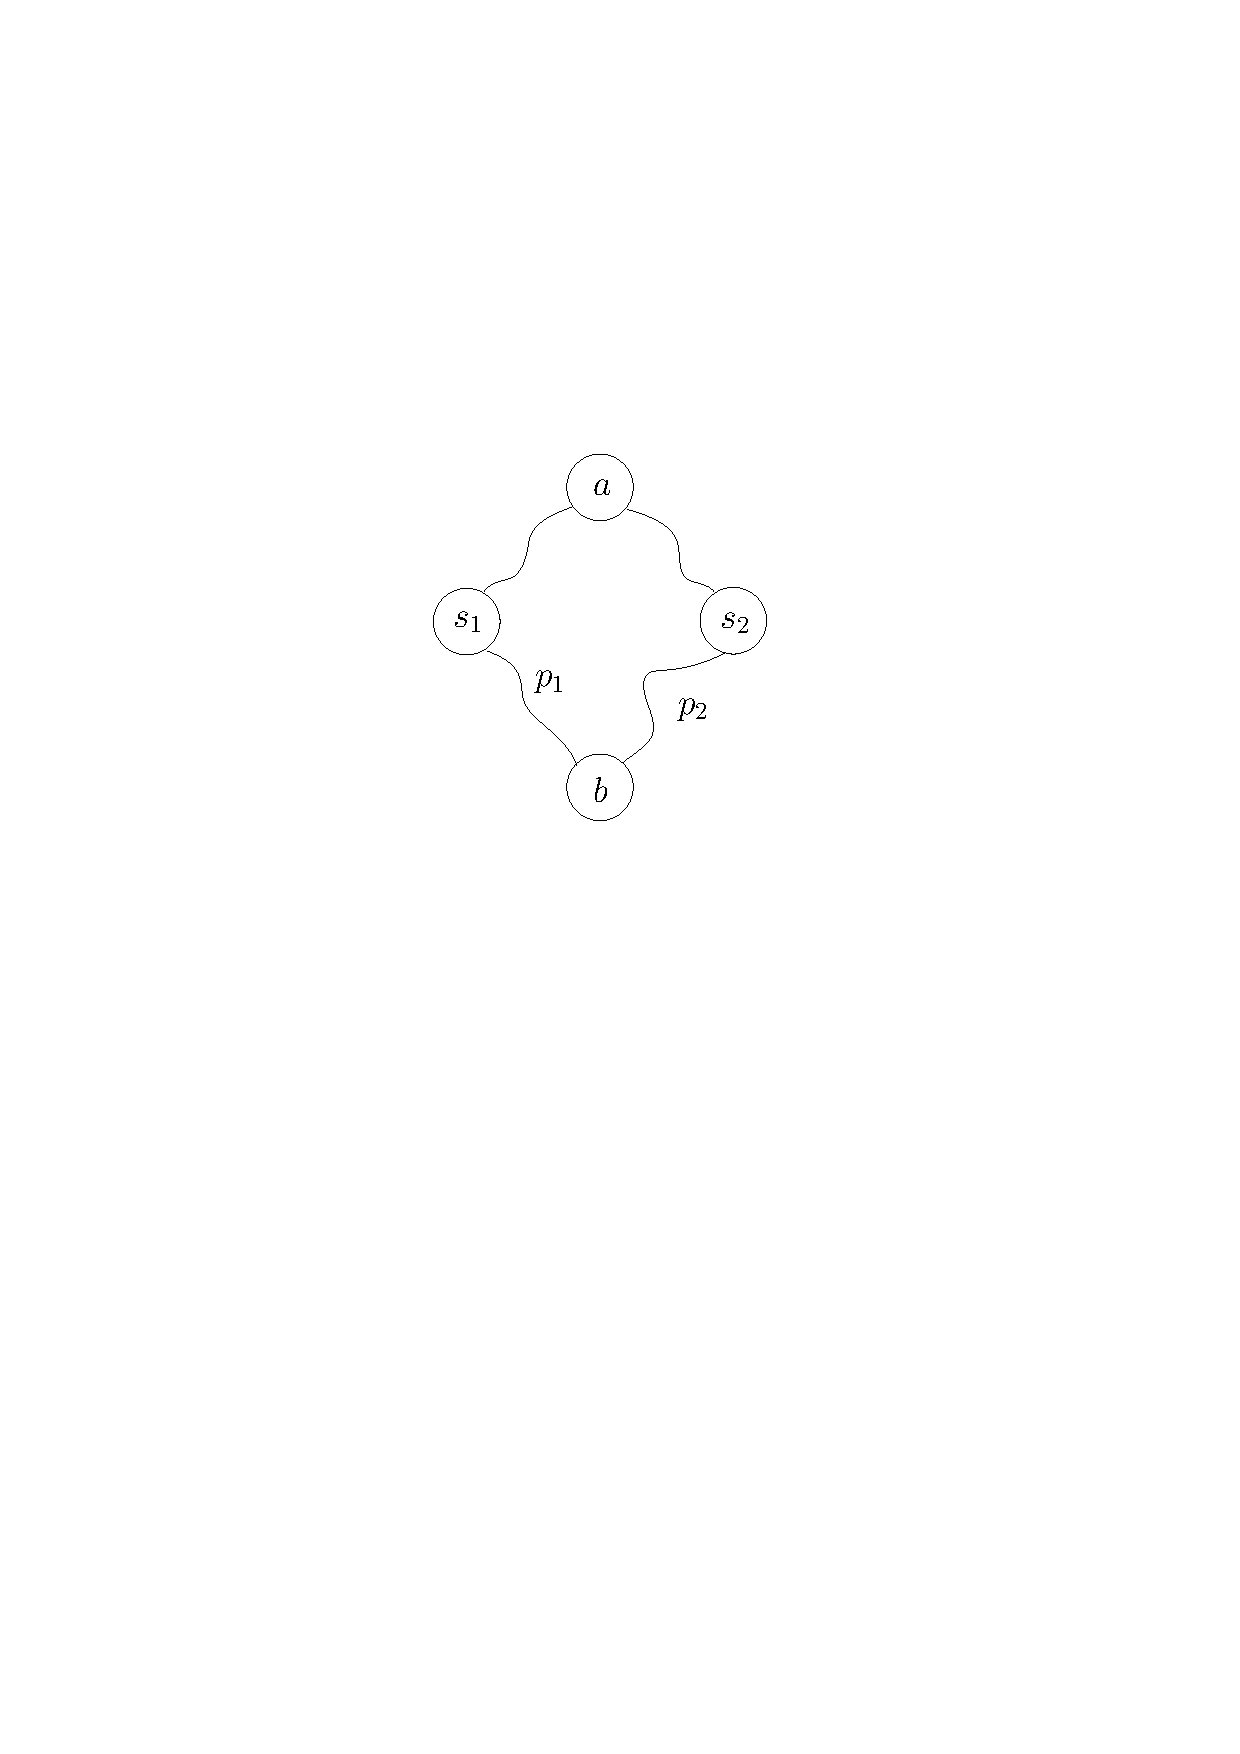
\includegraphics[page=1]{fig/03-2a-pfade}
\end{center}

Wir haben mind. zwei Knoten $s_1$ und $s_2$, die im Separator liegen und nicht-adjazent sind.

Es führen Pfade von a zu beiden Knoten. Diese Pfade müssen nicht wie im Bild dargestellt knotendisjunkt sein, aber das erleichtert die Vorstellung.

Von $s_1$ und $s_2$ gibt es die oben beschriebenen Pfade nach $b$, die keine anderen Knoten des Separators verwenden. Auch diese Pfade müssen nicht knotendisjunkt sein.

Allerdings gibt es hiermit mindestens 4 Knoten, die einen Kreis der Länge mind. 4 induzieren. Im Beispielbild sind das $a, s_1, b, s_2$. Falls die Pfade nicht knotendisjunkt sind, wählen wir anstatt von $a$ und $b$ einfach die letzte Stelle, an der sich die entsprechenden Pfade einen Knoten teilen.

Damit haben wir einen Widerspruch gefunden, denn nun kann der Graph nach Definition nicht mehr chordal sein.
Demnach müssen die Knoten aus S also eine Clique bilden.

\subexercise

Gegeben sei ein chordaler Graph $C = (V,E)$.

\emph{Fall 1}
Alle Knoten aus $C$ bilden eine Clique. Es gibt nichts zu tun.

\emph{Fall 2}
Die Knoten aus $C$ bilden keine Clique. Daraus folgt, dass es zwei verschiedene, nicht adjazente Knoten $v_1, v_2$ gibt.
Es bleibt zu zeigen, dass beide Knoten simplizial sind.

\emph{Fall 2.1}
$N(v_i)$ für $i \in \{1,2\}$ ist ein inklusionsmaximaler Separator, der der $v_1$ von $v_2$ trennt.
Mit Aufgabenteil~\ref{sec:sep-clique} wissen wir, dass $N(v_i)$ jeweils eine Clique sein muss. Damit sind die Knoten simplizial.

\emph{Fall 2.2}
$N(v_i)$ für $i \in \{1,2\}$ ist eine Clique. Damit sind beide Knoten simplizial.

\emph{Fall 2.3}
$N(v_i)$ für $i \in \{1,2\}$ ist ein kein inklusionsmaximaler Separator und bildet keine Clique. Wähle o.B.d.A $i = 1$.
Dann gibt es $S = N(v_i) \setminus M$ mit $S \neq \emptyset$ und $M \neq \emptyset$. S ist nun inklusionsmaximaler Separator.
$v_1$ kann also kein simplizialer Knoten sein. Wir müssen einen neuen Kandidaten finden.

Dazu betracten wir nun einen Knoten $x \in M$, der nicht mit allen Knoten aus $S$ verbunden ist. Solch ein Knoten muss existieren, da $S$ eine Clique ist, aber $N(v_1)$ nicht.

\emph{Fall 2.3.1}
$\exists s' \in S \colon \{x,s'\} \in E$. $x$ hat mind. eine Verbindung zum Seperator $S$.
Wir wählen nun $x$ als neues $v_1$ und wiederholen die Fallunterscheidung ab Fall 2 mit dem alten $v_2$ und $x$ als neues $v_1$.

\begin{center}
    \vspace{1ex}
    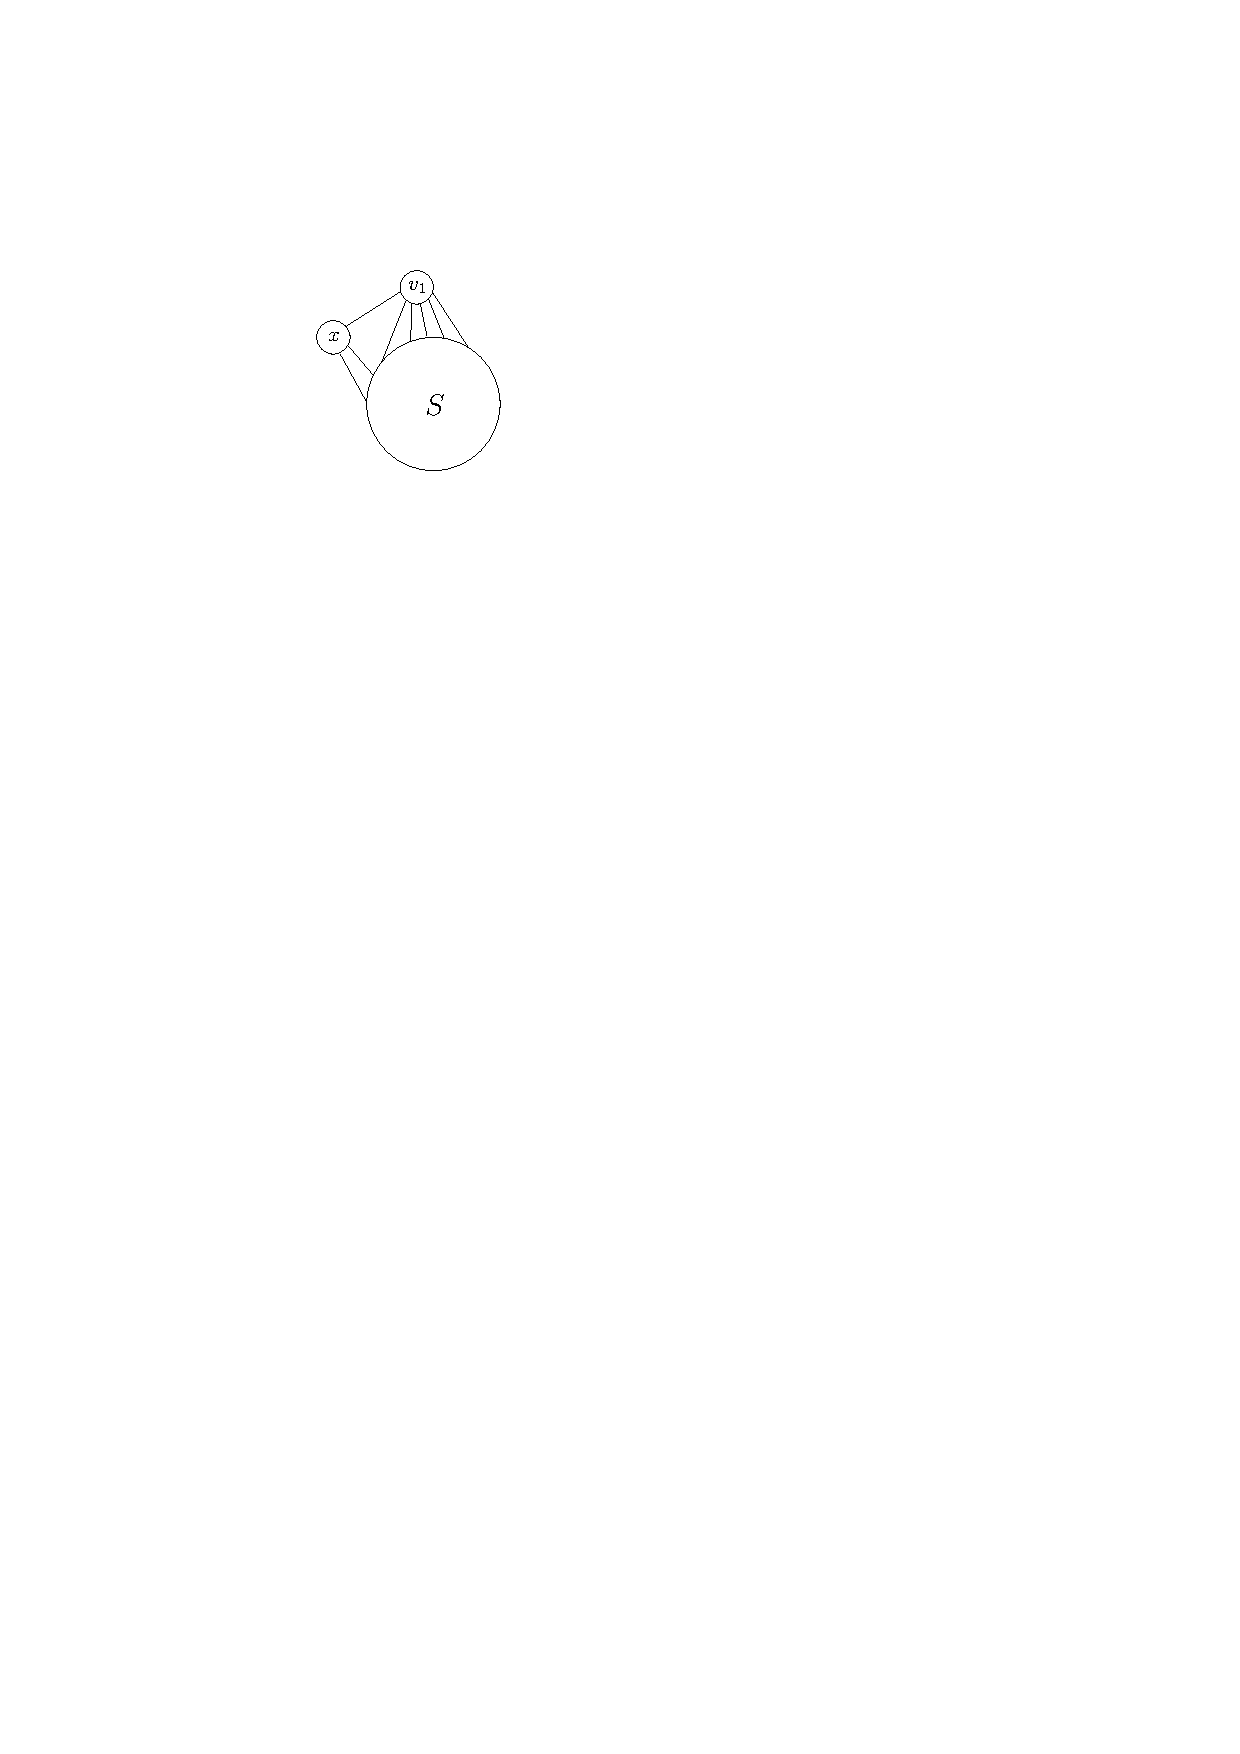
\includegraphics[page=1]{fig/03-2b-xtos}
\end{center}

Damit wird $N(x) \cap (S \cup \{v_1\})$ zu einem inklusionsmaximalen Seperator für $x$ und $v_2$.
Selbst wenn $x$ noch andere Verbindungen hat, können diese keine Pfade zu $v_2$ beinhalten, da $x$ sonst Teil von $S$ sein müsste.
Dadurch ändert sich die Nachbarschaft die wir betrachten. In dem Teilgraph in dem sich $v_1$ befindet, wenn man die Knoten aus $S$ aus $V$ entfernt, befinden sich nur endlich viele Knoten.
Da $x$ nicht mit allen Knoten aus $S$ verbunden ist, reduziert sich die Anzahl der relevanten Knoten in diesem Teilgraphen um mind. 1.

\emph{Fall 2.3.2}
$\nexists s' \in S \colon \{x,s'\} \in E$. $x$ hat keine Verbindung zum Seperator $S$.
Dann gehen wir analog vor und wählen $x$ als neues $v_1$.

Da $x$ nicht mit $S$ verbunden ist, reduziert sich also die Anzahl der Knoten im betrachteten Teilgraphen um mind. 1.

Schließlich müssen wir auf einen Knoten treffen, der in Fall 2.1 oder Fall 2.2 fällt, da sich in Fall 2.3 die Anzahl der betrachteten Knoten stets verringert.

Auf diese Weise finden wir immer zwei simpliziale Knoten.

\end{document}
